\chapter{Applications of Double Integrals}

\section{Total Mass and Charge}
Suppose there is a generic, thin layer (called a \textit{lamina}) with a 
variable density that occupies an area \textit{B} (see figure \ref{fig:lamina}).
Further, let the density of the lamina be described by a function, $\rho 
(x, y)$, which is continuous over \textit{B}. For some small rectangle centered
at $(x, y)$, the density is given by:
$$\rho (x, y) = \frac{\Delta m}{\Delta A}$$

where $\Delta m$ is the mass of the small rectangle and $\Delta A$ is the area.
Then the mass of the rectangle is given by:
$$\Delta m = \rho (x, y) \Delta A$$

\begin{figure}[htbp]
\centering
    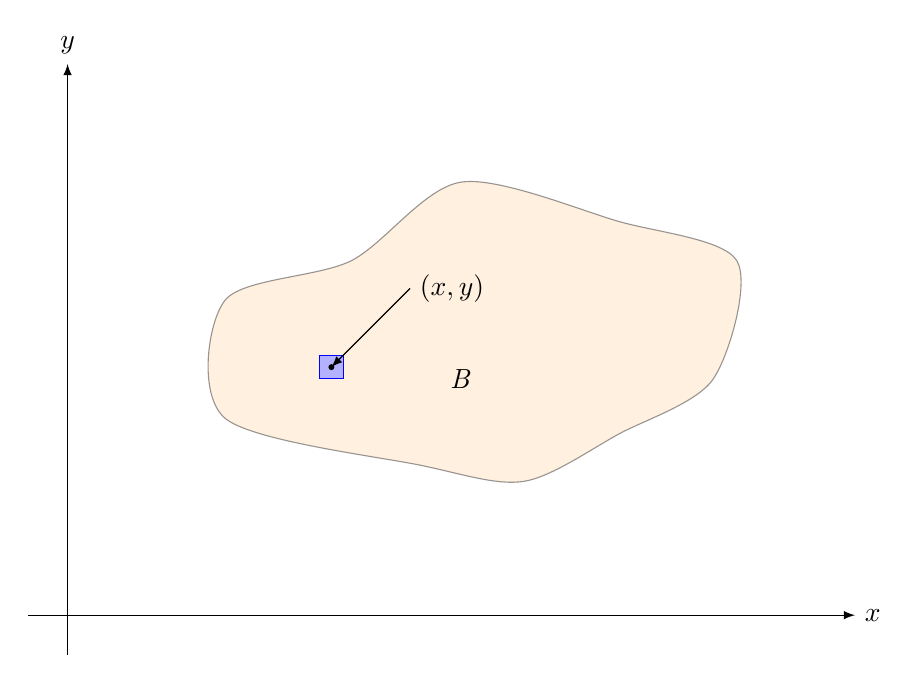
\begin{tikzpicture}
        \draw[-latex] (-0.5, 0) -- (10, 0) node[right] {$x$};
        \draw[-latex] (0, -0.5) -- (0, 7) node[above] {$y$};
        \draw[fill = orange!30, opacity = 0.4] plot [smooth cycle] 
        coordinates {(2, 2.5) (4.5, 1.9) (5.8, 1.7) (7, 2.3) (8.2, 3) 
        (8.5, 4.5) (7, 5) (5, 5.5) (3.6, 4.5) (2, 4)};
        \node[] at (5, 3) {\textit{B}};
        \draw[blue, fill = blue!30] (3.2, 3) rectangle (3.5, 3.3);
        \draw[fill = black] (3.35, 3.15) circle (0.03);
        \draw[latex-] (3.35, 3.15) -- (4.35, 4.15)  node[right] {$(x, y)$};
        
    \end{tikzpicture}
    \caption{A generic lamina that occupies the region \textit{B}}
    \label{fig:lamina}
\end{figure}

We can find the mass of the entire lamina by dividing it into many of these 
small rectangles and adding the masses of all the rectangles (see 
\ref{fig:laminagrid}). Just like in previous examples, there is some point 
$(x_{ij}^*, y_{ij}^*)$ in each rectangle, $R_{ij}$, such that the mass of the 
part of the lamina that occupies $R_{ij}$ is $\rho (x_{ij}^*, y_{ij}^*) \Delta 
A$. Adding all these masses yields:
$$m_{total} \approx \sum_{i = 1}^m \sum_{j = 1}^n \rho (x_{ij}^*, y_{ij}^*) 
\Delta A$$

Taking the limit as $m, n \to \infty$ increases the number of rectangles to 
yield the true total mass:
$$m_{total} = \lim_{m, n \to \infty} \sum_{i = 1}^m \sum_{j = 1}^n \rho (x_{ij
}^*, y_{ij}^*) \Delta A = \iint_{\textit{B}} \rho (x, y)\,dA$$

\begin{figure}[htbp]
\centering
    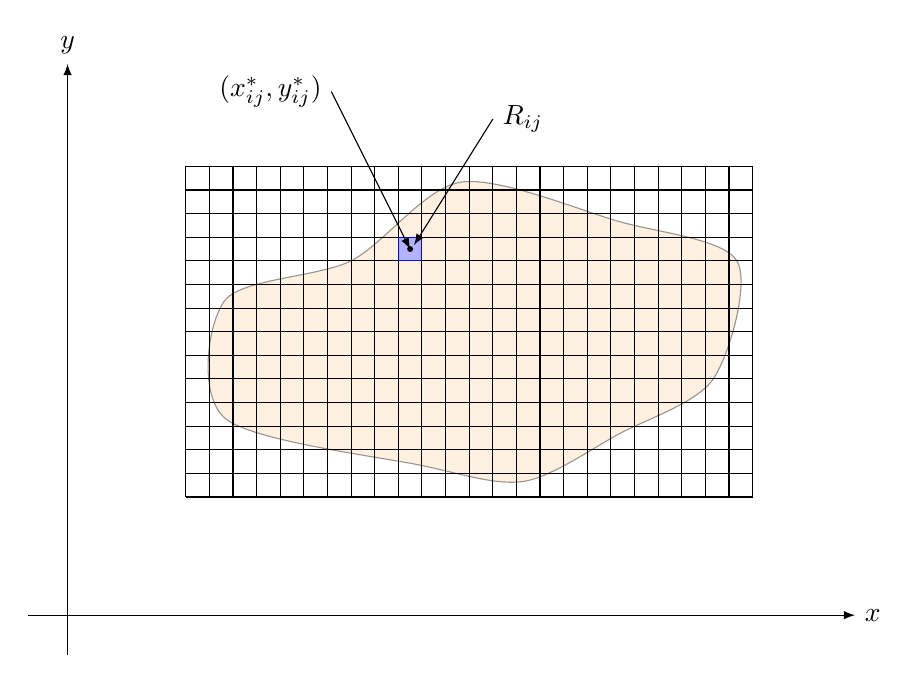
\begin{tikzpicture}
        \draw[-latex] (-0.5, 0) -- (10, 0) node[right] {$x$};
        \draw[-latex] (0, -0.5) -- (0, 7) node[above] {$y$};
        \draw[fill = orange!30, opacity = 0.4] plot [smooth cycle] 
        coordinates {(2, 2.5) (4.5, 1.9) (5.8, 1.7) (7, 2.3) (8.2, 3) 
        (8.5, 4.5) (7, 5) (5, 5.5) (3.6, 4.5) (2, 4)};
        \draw[step = 0.3] (1.5, 1.5) grid (8.7, 5.7);
        \draw[blue, fill = blue!30] (4.2, 4.5) rectangle (4.5, 4.8);
        \draw[fill = black] (4.35, 4.65) circle (0.03);
        \draw[latex-] (4.35, 4.65) -- (3.35, 6.65)  node[left] {$(x_{ij}^*, 
        y_{ij}^*)$};
        \draw[latex-] (4.4, 4.7) -- (5.4, 6.3) node[right] {$R_{ij}$};
        
    \end{tikzpicture}
    \caption{A generic lamina divided into many rectangles}
    \label{fig:laminagrid}
\end{figure}

\textbf{Example}: Find the total mass of a lamina that occupies the region 
$\textit{D} = \{ \left( x, y \right) \text{ }| \text{ } 1 \leq x \leq 3, 1 
\leq y \leq 4 \}$ with a density function $\rho (x, y) = 3y^2$. 

\textbf{Solution}: We know that the total mass is given by:
$$\iint_{\textit{D}} 3y^2\,dA$$

Applying Fubini's theorem, we see that:
$$\iint_{\textit{D}} 3y^2\,dA = \int_1^3 \int_1^4 3y^2\,dy\,dx$$
$$= \int_1^3 \left[ y^3 \right]_{y = 1}^{y = 4}\,dx = \int_1^3 \left[4^3 - 
1^3 \right]\,dx$$
$$= \int_1^3 63 \,dx = 63x|_{x = 1}^{x = 3} = 126$$

\begin{Exercise}[title = {Finding Total Mass}, label = total_mass]
Find the mass of the lamina that occupies the region, \textit{D}, and has the 
given density function, $\rho$. 
\begin{enumerate}
\item $\textit{D} = \{(x, y)\text{ }|\text{ } 0 \leq x \leq 4, 0 \leq y \leq 3 
\}; \rho (x, y) = 1 + x^2 + y^2$
\item \textit{D} is the triangular region with vertices $(0, 0)$, $(2, 1)$, 
$(0, 3)$; $\rho (x, y) = x + y$
\vspace{50mm}
\end{enumerate}
\end{Exercise}

\begin{Answer}[ref = total_mass]
\begin{enumerate}
    \item $\iint_{\textit{D}} \left(1 + x^2 + y^2 \right)\,dA = \int_0^4 
    \int_0^3 \left( 1  + x^2 + y^2 \right)\,dy\,dx$ $= \int_0^4 \left[y + x^2y 
    + \frac{1}{3}y^3 \right]_{y = 0}^{y = 3}\,dx$ $= \int_0^4 \left[ 3 + 3x^2 
    + \frac{1}{3}(3)^3 \right]\,dx$ $= \int_0^4 \left(12 + 3x^2 \right)\,dx$ 
    $= \left[ 12x + x^3 \right]_{x = 0}^{x = 4} = 12(4) + 4^3 = 112$
    \item First, let's visualize this region, since it isn't a rectangle:
    
    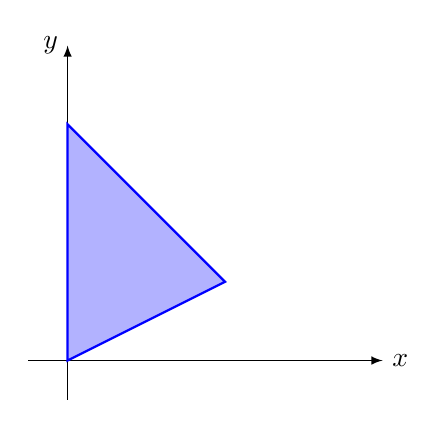
\begin{tikzpicture}
        \centering
        \draw[-latex] (-0.5, 0) -- (4, 0) node[right] {$x$};
        \draw[-latex] (0, -0.5) -- (0, 4) node[left] {$y$};
        \draw[thick, blue, fill = blue!30] (0,0) -- (2, 1) -- (0, 3) -- cycle;
    \end{tikzpicture}

    Let's divide the triangle horizontally and write equations for each of the 
    sides that do not lie on the $y$-axis.

    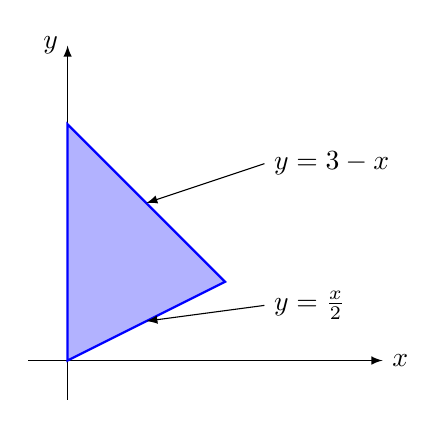
\begin{tikzpicture}
        \centering
        \draw[-latex] (-0.5, 0) -- (4, 0) node[right] {$x$};
        \draw[-latex] (0, -0.5) -- (0, 4) node[left] {$y$};
        \draw[thick, blue, fill = blue!30] (0,0) -- (2, 1) -- (0, 3) -- cycle;
        \draw[latex-] (1, 0.5) -- (2.5, 0.7) node[right] {$y = \frac{x}{2}$};
        \draw[latex-] (1, 2) -- (2.5, 2.5) node[right] {$y = 3 - x$};
    \end{tikzpicture}

    We see that we can describe region \textit{D} as $\textit{D} = \{ (x, y) 
    \text{ }|\text{ } 0 \leq x \leq 2, \frac{x}{2} \leq y \leq 3 - x\}$. 
    Therefore $\iint_{\textit{D}} \left( x + y \right) \,dA$ $= \int_0^3 \int_{
    x/2}^{3 - x} \left(x + y \right)\,dy\,dx$ $= \int_0^3 \left[xy + 
    \frac{1}{2} y^2 \right]_{y = x/2}^{y = 3 - x}\,dx$ $= \int_0^3 \left[ 
    \left(x(3 - x) \right) - \left(x (x/2) \right) + \frac{1}{2} \left( (3 - 
    x)^2 - (x/2)^2 \right) \right]\,dx$ 
    
    $= \int_0^3 \left[ \left(3x - x^2 - 
    \frac{x^2}{2} \right) + \frac{1}{2} \left( 9 - 6x + x^2 - \frac{x^2}{4} 
    \right) \right]\,dx$ $= \int_0^3 \left[-x^2 - \frac{x^2}{2} + \frac{x^2}{2}
    - \frac{x^2}{8} + 3x - 3x + \frac{9}{2} \right]\,dx$ $= \int_0^3 \left( -
    \frac{9x^2}{8} + \frac{9}{2} \right)\,dx$ $= \left[ \frac{9x}{2} -\frac{
    3x^3}{8} \right]_{x = 0}^{x = 2}$ $= \frac{9(2)}{2} - \frac{3(8)}{8} = 9 - 
    3 = 6$
\end{enumerate}
\end{Answer}

This method applies not only to mass density, but any other type of density. 
Some examples could include animals per acre of forest, cells per square 
centimeter of petri dish, or people per city block. A density physicists are 
often interested in is charge density (that is, the amount of charge, $Q$, per 
unit area). Charge is measured in coulombs (C). Often, charge density is given 
by a function, $\sigma (x, y)$, in units of coulombs per area (such as 
$\text{cm}^2$ or $\text{m}^2$). If there is some region, \textit{D}, with 
charge distributed across it such that the charge density can be described 
by a continuous function, $\sigma (x, y)$, then the total charge, Q, is given 
by:
$$Q = \iint_{\textit{D}} \sigma (x, y)\,dA$$

\textbf{Example}: Charge is distributed over the region \textit{B} shown in 
figure \ref{fig:charge} such that the charge density is given by $\sigma (x, y)
= xy$, measured in C/$\text{m}^2$. Find the total charge. 

\begin{figure}[htbp]
\centering
    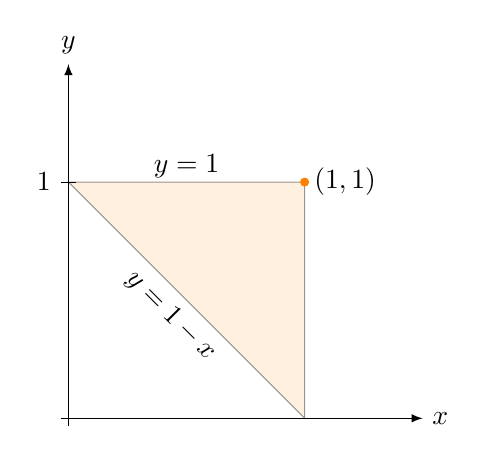
\begin{tikzpicture}
        \draw[-latex] (-0.1, 0) -- (4.5, 0) node[right] {$x$};
        \draw[-latex] (0, -0.1) -- (0, 4.5) node[above] {$y$};
        \draw[fill = orange!30, opacity = 0.4] (3, 0) -- (3, 3) -- (0, 3) -- 
        cycle;
        \draw[orange, fill = orange] (3, 3) circle (0.05) node[black, right] 
        {$(1, 1)$};
        \draw[] (0.1, 3) -- (-0.1, 3) node[left] {$1$};
        \node[] at (1.5, 3.2) {$y = 1$};
        \node[rotate = -45] at (1.3, 1.3) {$y = 1 - x$};
        
    \end{tikzpicture}
    \caption{A triangular region over which charge is distributed such that 
    $\sigma (x, y) = xy$}
    \label{fig:charge}
\end{figure}

\textbf{Solution}: We know that total charge is given by:
$$Q = \iint_{\textit{B}} xy\,dA$$ 

Examining figure \ref{fig:charge}, we see that:
$$\iint_{\textit{B}} xy\,dA = \int_0^1 \int_{1 - x}^1 xy\,dy\,dx$$
$$= \int_0^1 \frac{x}{2} \left[ y^2 \right]_{y = 1 - x}^{y = 1}\,dx = \int_0^1 
\frac{x}{2} \left[ 1^2 - \left( 1 - x \right)^2 \right]\,dx$$
$$= \frac{1}{2} \int_0^1 x \left(1 - 1 + 2x - x^2 \right)\,dx = \frac{1}{2} 
\int_0^1 x \left(2x - x^2 \right)\,dx$$
$$= \frac{1}{2} \int_0^1 2x^2 - x^3\,dx = \frac{1}{2} \left[ \frac{2}{3}x^3 - 
\frac{1}{4}x^4 \right]_{x = 0}^{x = 1} = \frac{1}{2} \left( \frac{2}{3} - 
\frac{1}{4} \right) = \frac{5}{24} \text{C}$$


\section{Center of Mass}
For a thin disk (lamina) of variable density in the $xy$-plane, the coordinates
of the center of mass, $(\overline{x}, \overline{y})$, are given by:
$$\overline{x} = \frac{1}{m} \iint_{\textit{D}} x \rho (x, y)\,dA$$
$$\overline{y} = \frac{1}{m} \iint_{\textit{D}} y \rho (x, y)\,dA$$

where $m$ is the total mass and $\rho$ is the density of the lamina as a 
function of $x$ and $y$. 

\textbf{Example}: Find the center of mass of a triangular lamina with vertices 
at $(0, 0)$, $(2, 0)$, and $(0, 1)$ and a density function $\rho (x, y) = 2 + 
x + 3y$. 

\textbf{Solution}: We begin by visualizing the region so we can determine if 
it is type I or type II:

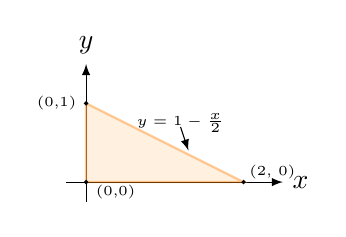
\begin{tikzpicture}
    \draw[-latex] (-0.25, 0) -- (2.5, 0) node[right] {$x$};
    \draw[-latex] (0, -0.25) -- (0, 1.5) node[above] {$y$};
    \draw[orange, thick, fill = orange!30, opacity = 0.4] (0,0) -- (2, 0) -- 
    (0, 1) -- cycle;
    \node[font = \tiny] at (1.2, 0.75) {$y = 1 - \frac{x}{2}$};
    \draw[-latex] (1.2, 0.7) -- (1.3, 0.4);
    \draw[black, fill = black] (0,1) circle (0.02cm) node[font = \tiny, left] 
    {(0,1)};
    \draw[black, fill = black] (0,0) circle (0.02cm) node[font = \tiny, right, 
    yshift = -0.13cm] {(0,0)};
    \draw[black, fill = black] (2, 0) circle (0.02cm) node[font = \tiny, right, 
    yshift = 0.13cm, xshift = -0.05cm] {(2, 0)};
\end{tikzpicture}

Recall that the total mass is given by $m = \iint_{\textit{D}} \rho (x, y)
\,dA$. As shown above, we can define $\textit{D} = \{ \left( x, y \right) | 0 
\leq x \leq 2, 0 \leq y \leq 1 - \frac{x}{2} \}$:
$$m = \int_{0}^{2} \int_{0}^{1 - x/2} \left( 2 + x + 3y \right) \,dy \,dx = 
\int_{0}^2 \left[2y + xy + \frac{3}{2}y^2 \right]_{y = 0}^{y = 1 - x/2}\,dx$$
$$= \int_0^2 \left[ 2(1 - \frac{x}{2}) + x(1 - \frac{x}{2}) + \frac{3}{2} (1 - 
\frac{x}{2})^2 \right]\,dx = \int_0^2 \left[ \frac{7}{2} - \frac{3x}{2} - 
\frac{x^2}{8} \right]\,dx$$
$$= \left[ \frac{7x}{2} - \frac{3x^2}{4} - \frac{x^3}{24} \right]_{x = 0}^{x = 
2} = \frac{7(2)}{2} - \frac{3(4)}{4} - \frac{8}{24} = 7 - 3 - \frac{1}{3} = 
\frac{11}{3}$$

Finding $\overline{x}$:
$$\overline{x} = \frac{1}{m} \iint_{\textit{D}} x \left( 2 + x + 3y \right) 
\,dA$$
$$\overline{x} = \frac{3}{11} \int_0^2 \int_0^{1 - x/2} \left[ 2x + x^2 + 3xy 
\right] \,dy \,dx$$
$$\overline{x} = \frac{3}{11} \int_0^2 \left[ 2xy + x^2y + \frac{3}{2}xy^2 
\right]_{y = 0}^{y = 1 - x/2} \,dx$$
$$\overline{x} = \frac{3}{11} \int_0^2 \left[ \frac{7x}{2} - \frac{3x^2}{2} - 
\frac{x^3}{8} \right]\,dx$$
$$\overline{x} = \frac{3}{11} \left[ \frac{7x^2}{4} - \frac{x^3}{2} - \frac{x
^4}{32} \right]_{x = 0}^{x = 2}$$
$$\overline{x} = \frac{3}{11} \left[ \frac{7(4)}{4} - \frac{8}{2} - \frac{16}{
32} \right] = \frac{3}{11} \left( 7 - 4 - \frac{1}{2} \right) = \frac{3}{11} 
\left( \frac{5}{2} \right) = \frac{15}{22}$$

We can similarly find $\overline{y}$:
$$\overline{y} = \frac{1}{m} \iint_{\textit{D}} y \left(2 + x + 3y \right)
\,dA$$
$$\overline{y} = \frac{3}{11} \int_0^2 \int_0^{1 - x/2} \left[ 2y + xy + 3y^2 
\right]\,dy\,dx$$
$$\overline{y} = \frac{3}{11} \int_0^2 \left[ y^2 + \frac{x}{2}y^2 + y^3 
\right]_{y = 0}^{y = 1 - x/2} \,dx$$
$$\overline{y} = \frac{3}{11} \int_0^2 \left[ \left(1 - \frac{x}{2} \right)^2 
+ \frac{x}{2} \left( 1 - \frac{x}{2} \right)^2 + \left( 1 - \frac{x}{2} \right)
^3 \right] \,dx$$
$$\overline{y} = \frac{3}{11} \int_0^2 \left[ 2 - 2x + \frac{x^2}{2} \right]
\,dx = \frac{3}{11} \left[ 2x - x^2 + \frac{x^3}{6} \right]_{x = 0}^{x = 2}$$
$$\overline{y} = \frac{3}{11} \left[ 2(2) - 2(2) + \frac{8}{6} \right] = \frac{
3}{11} \left( \frac{4}{3} \right) = \frac{4}{11}$$

Therefore, the center of mass $(\overline{x}, \overline{y})$ is $(\frac{15}{22
}, \frac{4}{11})$.

\begin{Exercise}[title = {Center of Mass}, label = c_of_m]
Find the center of mass of: 
\begin{enumerate}
\item A lamina that occupies the area enclosed by the 
curves $y = 0$ and $y = 2\sin{x}$ from $0 \leq x \leq \pi$ if its density is 
given by $\rho (x,y) = x$.
\item The region \textit{D} if $\textit{D} = \{(x, y)\text{ }|\text{ } 0 \leq x
\leq 4, 0 \leq y \leq 3 \}; \rho (x, y) = 1 + x^2 + y^2$
\item The triangular region \textit{D} with vertices $(0, 0)$, $(2, 1)$, 
$(0, 3)$; $\rho (x, y) = x + y$
\end{enumerate}
\vspace{100mm}
\end{Exercise}

\begin{Answer}[ref = c_of_m]
\begin{enumerate}
\item First, we find the total mass: $m = \int_0^{\pi} \int_0^{2\sin{x}} x \,dy
\,dx$ 
$= \int_0^{\pi} \left[ xy \right]_{y = 0}^{y = 2\sin{x}}\,dx$ $= \int_0^{\pi} 2
x\sin{x}\,dx$. 

We apply integration by parts to evaluate the integral: 
$\int_0^{\pi} 2x\sin{x}\,dx = \left(-2x \cos{x} \right)|_{x = 0}^{x = \pi} + 
\int_0^{\pi} 2 \cos{x}\,dx$ 
$= \left[-2 \pi (-1) \right] - \left( 0 \right) + \sin{x}|_{x = 0}^{x = \pi}$ 
$= 2\pi + \sin{\pi} - \sin{0} = 2\pi$

Now that we know $m = 2\pi$, we can find $\overline{x}$ and $\overline{y}$: 
$\overline{x} = \frac{1}{2\pi} \int_0^{\pi} \int_0^{2\sin{x}} x \cdot x \,dy 
\,dx$ 
$= \frac{1}{2\pi} \int_0^{\pi} x^2y|_{y = 0}^{y = 2\sin{x}}\,dx$ 
$= \frac{1}{2\pi} \int_0^{\pi} x^2 \left(2\sin{x} \right)\,dx$ 
$= \frac{1}{\pi} \int_0^{\pi} x^2 \sin{x}\,dx$. 

Applying integration by parts: $\frac{1}{\pi} \int_0^{\pi} x^2 \sin{x}\,dx$ 
$= \frac{1}{\pi} \left[ x^2 \left(-\cos{x} \right)|_{x = 0}^{x = \pi} - \int_0^
{\pi} 2x \left( -\cos{x} \right) \,dx \right]$ 
$= \frac{1}{\pi} \left[ \left( -\pi^2 \cos{\pi} \right) + 2\int_0^{\pi} x\cos{x
}\,dx \right]$ 
$= \frac{1}{\pi} \left[ \pi^2 + 2\int_0^{\pi} x\cos{x}\,dx \right]$ $= \pi + 
\frac{2}{\pi} \int_0^{\pi} x\cos{x}\,dx$. 

Applying integration by parts again: $\pi + \frac{2}{\pi} \int_0^{\pi} x\cos{x}
\,dx$ 
$= \pi + \frac{2x\sin{x}}{\pi}|_{x = 0}^{x = \pi} - \frac{2}{\pi} \int_0^{\pi} 
\sin{x}\,dx$
$= \pi -\frac{2}{\pi} \int_0^{\pi} \sin{x}\,dx$
$= \pi + \frac{2}{\pi} \left[ \cos{x} \right]_{x = 0}^{x = \pi}$
$= \pi + \frac{2}{\pi} \left[ \cos{\pi} - \cos{0} \right]$
$= \pi + \frac{2}{\pi} \left(-1 - 1 \right)$ $= \pi - \frac{4}{\pi} = 
\overline{x}$

And finding $\overline{y}$: 
$\overline{y} = \frac{1}{2\pi} \int_0^{\pi} \int_0^{2 \sin{x}} y \cdot x \,dy 
\,dx$
$= \frac{1}{2\pi} \int_0^{\pi} \left[ \frac{1}{2}xy^2 \right]_{y = 0}^{y = 2
\sin{x}} \,dx$
$= \frac{1}{4\pi} \int_0^{\pi} x \left[ 2\sin{x} \right]^2 \,dx$ 
$= \frac{1}{4\pi} \int_0^{\pi} 4x \sin^2{x}\,dx$ 
$= \frac{1}{\pi} \int_0^{\pi} x\sin^2{x}\,dx$ 
$=\frac{1}{\pi} \int_0^{\pi} x \frac{1-\cos{\left(2x\right)}}{2}\,dx$ 
$= \frac{1}{\pi} \int_0^{\pi} \frac{x}{2}\,dx - \frac{1}{\pi} \int_0^{\pi} x 
\cos{(2x)}\,dx$ 
$= \frac{1}{2\pi} \left[ \frac{x^2}{2} \right]_{x = 0}^{x = \pi} - \frac{1}{\pi
} \left[ \frac{1}{2}x\sin{(2x)}|_{x = 0}^{x = \pi} - \frac{1}{2} \int_0^{\pi} 
\sin{(2x)}\,dx \right]$
$= \frac{1}{2\pi} \left( \frac{\pi^2}{2} \right) - \frac{1}{2\pi} \left[ \pi
\sin{(2\pi)} - 0 + \frac{1}{2} \cos{(2x)}|_{x - 0}^{x = \pi} \right]$
$= \frac{\pi}{4} - \frac{1}{2\pi} \left[ \frac{1}{2} \left(\cos{2\pi} - \cos{0}
\right) \right] = \frac{\pi}{4}$

Therefore, the center of mass is found at $\left( \overline{x}, \overline{y}
\right) = \left( \pi - \frac{4}{\pi}, \frac{\pi}{4} \right)$

\item We know from a previous question that the total mass of this lamina is 
112 (see \textit{Finding Total Mass}). 

Finding $\overline{x}$: $\overline{x} = \frac{1}{112} \int_0^4 \int_0^3 x 
\left( 1 + x^2 + y^2 \right)\,dy\,dx$ 
$= \frac{1}{112} \int_0^4 \int_0^3 \left(x + x^3 + xy^2 \right)\,dy\,dx$ 

$= \frac{1}{112} \int_0^4 \left[ xy + x^3y + \frac{x}{3}y^3 \right]_{y = 0}^{y 
= 3} \,dx$ 
$= \frac{1}{112} \int_0^4 \left[3x + 3x^3 + 9x \right]\,dx$ 
$= \frac{3}{112} \int_0^4 \left[ 4x + x^3 \right]\,dx$ 
$= \frac{3}{112} \left[ 2x^2 + \frac{x^4}{4} \right]_{x = 0}^{x = 4}$ 
$= \frac{3}{112} \left[ 2(4)^2 - 2(0)^2 + \frac{4^4}{4} - \frac{0^4}{4} 
\right]$ 
$= \frac{3}{112} \left[ 32 + 64 \right] = \frac{3 \cdot 96}{112} = \frac{3 
\cdot 2 \cdot 2 \cdot 2 \cdot 2 \cdot 2 \cdot 3}{2 \cdot 2 \cdot 7 \cdot 2 
\cdot 2} = \frac{18}{7}$

Finding $\overline{y}$: $\overline{y} = \frac{1}{112} \int_0^4 \int_0^3 y 
\left( 1 + x^2 + y^2 \right)\,dy\,dx$ 
$= \frac{1}{112} \int_0^4 \int_0^3 \left[ y + x^2y + y^3 \right]\,y\,dx$ 

$= \frac{1}{112} \int_0^4 \left[ \frac{y^2}{2} + \frac{x^2y^2}{2} + \frac{y^4}{
4} \right]_{y = 0}^{y = 3} \,dx$ 
$= \frac{1}{112} \int_0^4 \left[ \frac{3^2}{2} + \frac{3^2x^2}{2} + \frac{3^4}{
4} \right]\,dx$ 
$= \frac{1}{112} \int_0^4 \left[ \frac{99}{4} + \frac{9}{2}x^2 \right] \,dx$ 
$= \frac{1}{112} \left[ \frac{99}{4}x + \frac{3}{2}x^3 \right]_{x = 0}^{x = 4}$ 
$= \frac{3}{224} \left[\frac{33}{2}(4) + 4^3 \right]$ 
$= \frac{3}{224} \left( 66 + 64 \right) = \frac{3 \cdot 130}{224} = \frac{3 
\cdot 65}{112} = \frac{195}{112}$

Therefore, the center of mass of the rectangular region \textit{D} is $\left(
\frac{18}{7}, \frac{195}{112} \right)$

\item We know from a previous question (see \textit{Finding Total Mass}) that 
the total mass of \textit{D} is 6, and it can be described as $\textit{D} = \{ (
x, y) \text{ }|\text{ } 0 \leq x \leq 2, \frac{x}{2} \leq y \leq 3 - x\}$

Finding $\overline{x}$:

$\overline{x} = \frac{1}{6} \int_0^2 \int_{x/2}^{3 - x} x \left(x + y \right)
\,dy\,dx$
$= \frac{1}{6} \int_0^2 \int_{x/2}^{3 - x} \left(x^2 + xy \right)\,dy\,dx$
$= \frac{1}{6} \int_0^2 \left[ x^2y + \frac{x}{2}y^2 \right]_{y = x/2}^{y = 3 -
x}\,dx$
$= \frac{1}{6} \int_0^2 \left[ x^2\left( 3 - x - \frac{x}{2} \right) + \frac{x
}{2}\left( \left( 3 - x \right)^2 - \left( \frac{x}{2} \right)^2 \right) 
\right]\,dx$
$= \frac{1}{6} \int_0^2 \left[ 3x^2 - x^3 - \frac{x^3}{2} + \frac{x}{2} \left(
9 - 6x + x^2 - \frac{x^2}{4} \right) \right]\,dx$
$= \frac{1}{6} \int_0^2 \left[ 3x^2 - \frac{3}{2}x^3 + \frac{x}{2} \left( 9 - 
6x + \frac{3}{4}x^2 \right) \right]\,dx$
$= \frac{1}{6} \int_0^2 \left[ 3x^2 - \frac{3}{2}x^3 + \frac{9}{2}x - 3x^2 + 
\frac{3}{8}x^3 \right]\,dx$
$= \frac{1}{6} \int_0^2 \left[ \frac{9}{2}x - \frac{9}{8}x^3 \right]\,dx$
$= \frac{1}{6} \left[ \frac{9}{4}x^2 - \frac{9}{32}x^4 \right]_{x = 0}^{x = 2}$
$= \frac{1}{6} \left[ \frac{9 \cdot 4}{4} - \frac{9 \cdot 16}{32} \right]$
$= \frac{1}{6} \left[9 - \frac{9}{2} \right] = \frac{1}{6} \cdot \frac{9}{2} = 
\frac{9}{12} = \frac{3}{4}$

And finding $\overline{y}$:

$\overline{y} = \frac{1}{6} \int_0^2 \int_{x/2}^{3 - x} y \left(x + y \right)
\,dy\,dx$
$= \frac{1}{6} \int_0^2 \int_{x/2}^{3-x} \left(xy + y^2 \right)\,dy\,dx$
$= \frac{1}{6} \int_0^2 \left[ \frac{x}{2}y^2 + \frac{1}{3}y^3 \right]_{y = x/2
}^{y = 3 - x}\,dx$
$= \frac{1}{6} \int_0^2 \left[ \frac{x}{2} \left( \left( 3 - x \right)^2 - 
\left( \frac{x}{2} \right)^2 \right) + \frac{1}{3} \left( \left( 3 - x \right)^
3 - \left( \frac{x}{2} \right)^3 \right) \right]\,dx$

$= \frac{1}{6} \int_0^2 \left[ \frac{x}{2} \left( 9 - 6x + x^2 - \frac{x^2}{4} 
\right) + \frac{1}{3} \left( 27 - 27x +9x^2 - x^3 - \frac{x^3}{8} \right) 
\right]\,dx$

$= \frac{1}{6} \int_0^2 \left[ \frac{x}{2} \left( 9 - 6x + \frac{3x^2}{4} 
\right) + \frac{1}{3} \left( 27 - 27x + 9x^2 - \frac{9x^3}{8} \right) \right]
\,dx$

$= \frac{1}{6} \int_0^2 \left[ \frac{9}{2}x - 3x^2 + \frac{3}{8}x^3 + 9 - 9x + 
3x^2 - \frac{3}{8}x^3 \right]\,dx$
$= \frac{1}{6} \int_0^2 \left[ 9 - \frac{9}{2}x  \right]\,dx$
$= \frac{1}{6} \left[ 9x - \frac{9}{4}x^2 \right]_{x = 0}^{x = 2}$
$= \frac{3}{6} \left[3(2) - \frac{3}{4}(2)^2 \right]$
$= \frac{1}{2} \left(6 - 3 \right) = \frac{1}{2} \cdot 3 = \frac{3}{2}$

Therefore, the center of mass is $\left( \overline{x}, \overline{y} \right) = 
\left( \frac{3}{4}, \frac{3}{2} \right)$
\end{enumerate}

\end{Answer}

\section{Moment of Inertia}
We can also use double integrals to find the \textbf{moment of inertia}\index{
moment of inertia} of a lamina about a particular axis (we will extend this to 
three-dimensional objects in the next chapter on triple integrals). Recall that the
moment of inertia for a particle with mass \textit{m} a distance \textit{r} 
from the axis of rotation is $mr^2$. Dividing a lamina into small pieces, we 
see that the moment of inertia of each piece about the $x$-axis is:
$$\left( y_{ij}^* \right)^2 \rho \left( x_{ij}^* , y_{ij}^* \right) \Delta A$$

Where $x_{ij}^*$ and $y_{ij}^*$ are the $x$- and $y$-coordinates of the small 
piece. The moment of inertia of the entire lamina about the $x$-axis is then 
the sum of all the individual moments:
$$I_x = \sum_{i = 1}^n \sum_{j = 1}^n \left( y_{ij}^* \right)^2 \rho \left( x_{
ij}^* , y_{ij}^* \right) \Delta A = \iint_{\textit{D}} y^2 \rho \left(x, y 
\right) \,dA$$

Similarly, the moment of inertia of a lamina about the $y$-axis is:
$$I_y = \sum_{i = 1}^n \sum_{j = 1}^n \left( x_{ij}^* \right)^2 \rho \left( x_{
ij}^* , y_{ij}^* \right) \Delta A = \iint_{\textit{D}} x^2 \rho \left(x, y 
\right) \,dA$$

\textbf{Example}: Find the moment of inertia of a square centered at the origin
with side length $r$ and constant density $\rho$ about the $x$-axis.

\textbf{Solution}: We can describe the square as the region bounded by $
\textit{D} = \{(x, y)| -r/2 \leq x \leq r/2, -r/2 \leq y \leq r/2 \}$ with 
density function $\rho(x, y) = \rho$. Therefore, the moment of inertia about 
the $x$-axis is given by:
$$I_x = \int_{-r/2}^{r/2} \int_{-r/2}^{r/2} \rho y^2 \,dy\,dx$$
$$= \rho \int_{-r/2}^{r/2} \left[ \frac{1}{3} y^3 \right]_{y = -r/2}^{y = r/2} 
\,dx$$
$$= \frac{\rho}{3} \int_{-r/2}^{r/2} \left[ \frac{r^3}{8} - \left( -\frac{r^3}{
8} \right) \right]\,dx$$
$$= \frac{\rho}{3} \int_{-r/2}^{r/2} \left[ \frac{r^3}{4} \right]\,dx = \frac{
r^3 \rho}{12} \int_{-r/2}^{r/2} 1\,dx$$
$$= \frac{r^3 \rho}{12} \left[ x \right]_{x = -r/2}^{x = r/2} = \frac{r^3 \rho
}{12} \cdot r = \frac{r^4 \rho}{12}$$

We can also find the moment of inertia about the origin, $I_o$. This is the 
moment of inertia for an object rotating in the $xy$-plane about the origin. 
The moment of inertia about the origin is the sum of the moments of inertia 
about the $x$- and $y$-axes:
$$I_o = I_x + I_y = \iint_{\textit{D}} \left( x^2 + y^2 \right) \rho(x, y)\,
dA$$

\textbf{Example}: Find the moment of inertia about the origin of a disk with 
density $\rho(x, y) = b$, centered at the origin, with a radius of $a$. Show that 
this is equal to the expected moment of inertia, $\frac{1}{2}MR^2$, where $M$ 
is the total mass of the disk and $R$ is the radius of the disk.

\textbf{Solution}: Since we are examining a circle about the origin, the 
region can be described in polar coordinates as $\textit{D} = \{(r, \theta)
\text{ }|\text{ } 0 \leq r \leq a, \text{ }0 \leq \theta \leq 2\pi \}$. 
Converting from Cartesian coordinates to polar coordinates:
$$I_o = \iint_{\textit{D}} \left(x ^2 + y^2 \right) b\,dA = \int_0^a \int_0^{2
\pi} r \left( r^2 \right) b\,d\theta \,d r$$
$$= \int_0^a r^3\,dr \cdot \int_0^{2\pi}b \,d\theta = \frac{a^4}{4} \cdot 
\left(2\pi b \right) = \frac{\pi a^4 b}{2}$$

The total mass of this disk is the density, $b$, multiplied by the area, $\pi 
a^2$. Therefore,
$$R = a$$
$$M = \pi a^2 b$$

Substituting into the result of our double integral, we see that:
$$\frac{\pi a^4 b}{2} = \left( \pi a^2 b \right) \cdot \left( \frac{a^2}{2} 
\right) = M \cdot \frac{R^2}{2} = \frac{1}{2}MR^2$$

\subsection{Radius of Gyration}
When modeling rotating objects, it can be helpful to have a simplified model. 
A spinning, continuous object can be modeled as a point mass by using the 
lamina's \textit{radius of gyration}\index{radius of gyration}. The radius of 
gyration of a lamina about the origin is a radius, $R$, such that:
$$mR^2 = I_o$$

where $m$ is the mass of the lamina and $I$ is the moment of inertia of the 
lamina. Essentially, we are finding a radius such that if the lamina were 
shrunk down to a point mass and rotated about the axis at that radius, the 
moment of inertia would be the same. 

We can also find radii of gyration about the $x$- and $y$-axes:
$$m \overline{\overline{y}}^2 = I_{x}$$
$$m \overline{\overline{x}}^2 = I_{y}$$

About the origin, $R = \sqrt{ \overline{\overline{x}}^2 + \overline{\overline{y}}^2}$. 

\textbf{Example}: Find the radius of gyration about the $y$-axis for a disk 
with density $\rho(x, y) = y$ if the disk has radius 2 and is centered at $(0, 
2)$. 

\textbf{Solution}: We are ultimately looking for a radius such that $m
\overline{\overline{x}}^2 = I_y$, so we need to know the mass, $m$, and the 
moment of inertia about the $y$-axis, $I_y$. First, let's find the total mass, 
$m$, of the disk. We can describe the disk in polar coordinates as $\textit{D} 
= \{(r, \theta)\text{ }|\text{ }0 \leq r \leq 4\sin{\theta}, 0 \leq \theta 
\leq \pi\}$, and therefore the mass is given by:
$$m = \iint_{\textit{D}} y \,dA = \int_0^{\pi} \int_0^{4\sin{\theta}} r \left(r
\sin{\theta} \right)\,dr \,d\theta$$
$$= \int_0^{\pi} \sin{\theta} \int_0^{4\sin{\theta}} r^2\,dr\,d\theta = \frac{1
}{3} \int_0^{\pi} \sin{\theta} \left[ 4\sin{\theta} \right]^3\,d\theta$$
$$= \frac{64}{3} \int_0^{\pi} \sin^4{\theta}\,d\theta = \frac{64}{3} \int_0^{
\pi} \left( \frac{1 - \cos{2\theta}}{2} \right)^2\,d\theta = \frac{64}{3} 
\left( \frac{1}{2} \right)^2 \int_0^{\pi} \left( 1 - 2\cos{2\theta} + \cos^2{2
\theta}\right) \,d\theta$$
$$= \frac{16}{3} \left[ \left(\theta - \sin{2\theta} \right)_{\theta = 0}^{
\theta = \pi} + \int_0^{\pi} \frac{1 + \cos{4\theta}}{2} \,d\theta \right] = 
\frac{16}{3} \left[ \pi + \frac{1}{2} \left(\theta + \frac{1}{4}\sin{4\theta} 
\right)_{\theta = 0}^{\theta = \pi} \right]$$
$$= \frac{16}{3} \left[ \pi + \frac{\pi}{2} \right] = \frac{16}{3} \left( 
\frac{3\pi}{2} \right) = 8\pi$$

Now that we have found the mass, let's find the moment of inertia, $I_y$:
$$I_y = \iint_{\textit{D}} x^2 y\,dA = \int_0^{\pi} \int_0^{4\sin{\theta}} r 
\left(r \cos{\theta} \right)^2 \left(r \sin{\theta} \right)\,dr\,d\theta$$
$$= \int_0^{\pi} \left[ \cos^2{\theta} \sin{\theta} \int_0^{4\sin{\theta}} r^4 
\,dr \right]\,d\theta = \int_0^{\pi} \cos^2{\theta} \sin{\theta} \left[\frac{1
}{5}r^5 \right]_{\theta = 0}^{\theta = 4\sin{\theta}}\,d\theta$$
$$= \frac{1024}{5} \int_0^{\pi} \cos^2{\theta} \sin^6{\theta}\,d\theta = \frac{
1024}{5} \int_0^{\pi} \left( \frac{1 + \cos{2\theta}}{2} \right) \left( \frac{1
 - \cos{2\theta}}{2} \right)^3\,d\theta$$
$$= \frac{1024}{5} \left(\frac{1}{2} \right)^4 \int_0^{\pi} \left(1 + \cos{2
\theta} \right) \left( 1 - \cos{2\theta} \right) \left(1 - \cos{2\theta} 
\right)^2\,d\theta$$
$$= \frac{64}{5} \int_0^{\pi} \left(1 - \cos^2{2\theta} \right) \left(1 - 2
\cos{2\theta} + \cos^2{2\theta} \right)\,d\theta$$
$$= \frac{64}{5} \int_0^{\pi} 1 - 2\cos{2\theta} + \cos^2{2\theta} - \cos^2{2
\theta} + 2\cos^3{2\theta} - \cos^4{2\theta} \,d\theta$$
$$= \frac{64}{5} \int_0^{\pi} 1 - 2\cos{2\theta} + 2\cos{2\theta} \left(1 - 
\sin^2{2\theta} \right) - \left( \frac{1 + \cos{4\theta}}{2} \right)^2\,d
\theta$$
$$= \frac{64}{5} \int_0^{\pi} 1 + 2\cos{2\theta}\sin^2{2\theta} - \frac{1}{4} 
\left(1 + 2\cos{4\theta} + \cos^2{4\theta} \right)\,d\theta$$
$$= \frac{64}{5} \int_0^{\pi} 1 + 2\cos{2\theta}\sin^2{2\theta} - \frac{1}{4} 
- \frac{\cos{4\theta}}{2} - \frac{1}{4}\left( \frac{1 + \cos{8\theta}}{2} 
\right)\,d\theta$$
$$= \frac{64}{5} \left[\frac{5\theta}{8} + \frac{1}{3}\sin^3{\theta} - \frac{
\sin{4\theta}}{8} - \frac{\sin{8\theta}}{64} \right]_{\theta = 0}^{\theta = \pi
} = \frac{64}{5} \cdot \frac{5\pi}{8} = 8\pi$$

We have found that $m = 8\pi$ and $I_y = 8\pi$. Substituting to find the radius
of gyration:
$$m\overline{\overline{x}}^2 = I_y$$
$$(8\pi)\overline{\overline{x}}^2 = 8\pi$$
$$\overline{\overline{x}} = 1$$

Therefore, the radius of gyration about the $y$-axis is $\overline{\overline{x}
} = 1$

\begin{Exercise}[title = {Moments of Inertia and Radii of Gyration}, label = 
moment]
Find the requested moment of inertia and radius of gyration of the lamina with 
the given density function. 
\begin{enumerate}
\item about the $x$-axis, $\textit{D} = \{(x, y)\text{ }|\text{ } 1 \leq x \leq
4,\text{ } 0 \leq y \leq 3\}$, $\rho(x, y) = xy$.
\item about the $y$-axis, \textit{D} is enclosed by the curves $y = 0$ and $y =
2\cos{x}$ for $-\pi/2 \leq x \leq \pi/2$, $\rho(x, y) = x$.
\item about the origin, $\textit{D} = \{(r, \theta)\text{ }|\text{ }1 \leq r 
\leq 2, \text{ }0 \leq \theta \leq \pi\}$, $\rho(r, \theta) = r$. 
\end{enumerate}
\vspace{100mm}
\end{Exercise}

\begin{Answer}[ref = moment]
\begin{enumerate}
\item $$I_x = \iint_{\textit{D}} y^2 \rho(x, y)\,dA = \int_1^4 \int_0^3 y^2 (xy
) \,dy\,dx$$
$$= \int_1^4 \int_0^3 xy^3\,dy\,dx = \int_1^4 x \left[ \frac{1}{4} y^4 \right]_
{y = 0}^{y = 3}\,dx = \frac{1}{4} \int_1^4 81x\,dx$$
$$= \frac{81}{4} \left[ \frac{1}{2} x^2 \right]_{x = 1}^{x = 4} = \frac{81}{2} 
\left(4^2 - 1^2 \right) = \frac{81}{2} \cdot 15 = \frac{1215}{2}$$

To find the radius of gyration, first we need to find the total mass:
$$m = \iint_{\textit{D}} \rho(x, y)\,dA = \int_1^4 \int_0^3 xy\,dy\,dx$$
$$= \int_1^4 \frac{x}{2} \left[y^2 \right]_{y = 0}^{y = 3} \,dx = \frac{9}{2} 
\int_1^4 x\,dx = \frac{9}{2} \cdot \left( \frac{1}{2} \right) \cdot \left[x^2 
\right]_{x = 1}^{x = 4} = \frac{9}{4} \left[16 - 1 \right] = \frac{135}{2}$$

Finding the radius of gyration about the $x$-axis:
$$I_x = m\overline{\overline{y}}^2$$
$$\frac{1215}{2} = \left( \frac{135}{2} \right) \overline{\overline{y}}^2$$
$$9 = \overline{\overline{y}}^2$$
$$\overline{\overline{y}} = 3$$

\item $$I_y = \iint_{\textit{D}} x^2 \rho(x, y)\,dA = \int_{-\pi/2}^{\pi/2} 
\int_0^{2\cos{x}} x^2y\,dy\,dx$$
$$= \int_{-pi/2}^{\pi/2} x^2 \left[ \frac{1}{2}y^2 \right]_{y = 0}^{y = 2\cos{x
}}\,dx = \frac{1}{2} \int_{-\pi/2}^{\pi/2} x^2 \left(2\cos{x} \right)^2\,dx$$
$$= 2 \int_{-\pi/2}^{\pi/2} x^2 \cos^2{x}\,dx = 2\int_{-\pi/2}^{\pi/2} x^2 
\left( \frac{1 + \cos{2x}}{2} \right)\,dx = \int_{-\pi/2}^{\pi/2}x^2\,dx + \int
_{-\pi/2}^{\pi/2} x^2 \cos{2x} \,dx$$
$$= \frac{1}{3} \left[ x^3 \right]_{x = -\pi/2}^{x = \pi/2} + \frac{1}{2}x^2
\sin{2x}|_{x = -\pi/2}^{x = \pi/2} - \int_{-\pi/2}^{\pi/2} \frac{1}{2}\sin{2x} 
\left(2x \right)\,dx$$
$$= \frac{1}{3} \left[ \left( \frac{\pi}{2} \right)^3 - \left( \frac{-\pi}{2} 
\right)^3 \right] - \int_{-\pi/2}^{\pi/2} x \sin{2x}\,dx$$
$$ = \frac{1}{3} \left( \frac{2\pi^3}{8} \right) - \left( \left[ -\frac{1}{2}x
\cos{2x} \right]_{x = -\pi/2}^{\pi/2} - \int_{-\pi/2}^{\pi/2} (-\frac{1}{2}
\cos{2x}) \,dx\right)$$
$$ = \frac{\pi^3}{12} + \left( \frac{1}{2} \left( \frac{\pi}{2} \right) \cos{(
\pi)} - \frac{1}{2} \left( \frac{-\pi}{2} \right) \cos{(-\pi)} \right) - \left[
\frac{1}{4} \sin{2x} \right]_{x = -\pi/2}^{\pi/2}$$
$$= \frac{\pi^3}{12} + \frac{\pi}{4}(-1) + \frac{\pi}{4}(-1) = \frac{\pi^3}{12}
- \frac{\pi}{2}$$

In order to find the radius of gyration, we need to first know the total mass:
$$m = \iint_{\textit{D}} \rho(x, y)\,dA = \int_{-\pi/2}^{\pi/2} \int_{0}^{2
\cos{x}} y \,dy\,dx$$
$$= \int_{-\pi/2}^{\pi/2} \frac{1}{2}y^2|_{y = 0}^{y = 2\cos{x}}\,dx = 
\frac{1}{2} \int_{-\pi/2}^{\pi/2} 4\cos^2{x}\,dx = \int_{-\pi/2}^{\pi/2} 1 + 
\cos{2x}\,dx$$
$$= \left[x + \frac{1}{2}\sin{2x} \right]_{x = -\pi/2}^{\pi/2} = \pi$$

We can then find the radius of gyration about the $y$-axis:
$$m \overline{\overline{x}}^2 = I_y$$
$$\pi \overline{\overline{x}}^2 = \frac{\pi^3}{12} - \frac{\pi}{2}$$
$$\overline{\overline{x}} = \sqrt{\frac{\pi^2}{12} - \frac{1}{2}}$$

\item $$I_o = \iint_{\textit{D}} \left( x^2 + y^2 \right) \rho(x, y) = \int_1^2
\int_0^{\pi} r (r^2) r \,d\theta \,dr$$
$$= \int_1^2 r^4 \theta|_{\theta = 0}^{\theta = \pi}\,dr = \pi \int_1^2 r^4\,dr
= \frac{\pi}{5} r^5|_{r = 1}^{r = 2} = \frac{\pi}{5} \left(2^5 - 1 \right) = 
\frac{\pi}{5} (31) = \frac{31\pi}{5}$$

We find the total mass:
$$m = \iint_{\textit{D}} \rho(x,y)\,dA = \int_1^2 \int_0^{\pi} r^2\,d\theta\,dr
= \int_1^2 r^2 \theta|_{\theta = 0}^{\theta = \pi}\,dr$$
$$= \pi \int_1^2 r^2\,dr = \frac{\pi}{3} r^3|_{r = 1}^{r = 2} = \frac{\pi}{3} 
\left(2^3 - 1 \right) = \frac{\pi}{3}(7) = \frac{7\pi}{3}$$

To find the radius of gyration about the origin:
$$mR^2 = I_o$$
$$\left( \frac{7\pi}{3} \right) R^2 = \frac{31\pi}{5}$$
$$R^2 = \frac{31}{5} \cdot \frac{3}{7} = \frac{93}{35}$$
$$R = \sqrt{\overline{\overline{x}}^2 + \overline{\overline{y}}^2} = \sqrt{
\frac{93}{35}}$$
\end{enumerate}
\end{Answer}

\section{Surface Area}
We have already seen how to find the areas of surfaces of revolution using 
single-variable calculus. Now, we will use multivariable calculus to find the 
surface area of a generic, two-variable function, $z = f(x, y)$. Suppose a 
surface, $S$, is defined by the continuous, partially differentiable function, 
$f(x, y)$, over a rectangular region, $R$ (see figure \ref{fig:surface}). 

\begin{figure}[htbp]
    \centering
    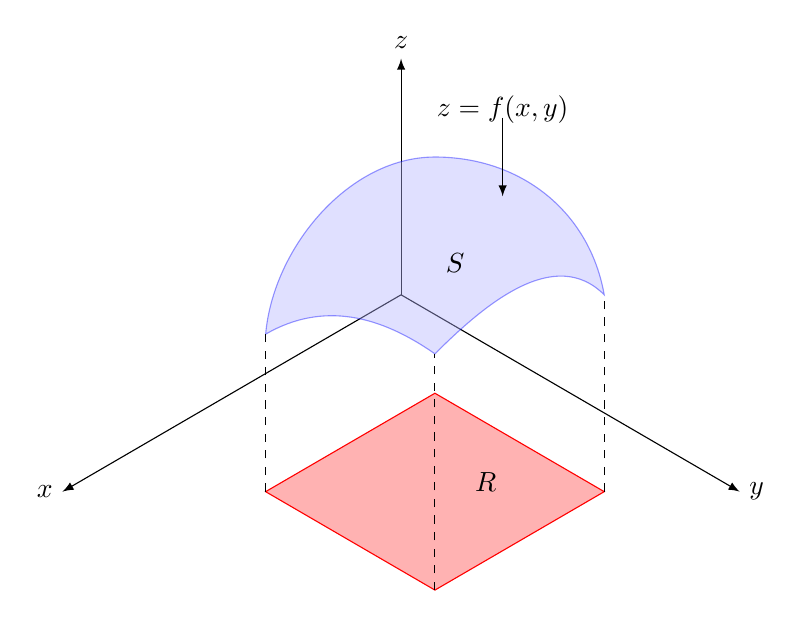
\begin{tikzpicture}[x = {(-0.86cm, -0.5cm)}, y = {(0.86cm, -0.5cm)}, 
    z = {(0cm, 1cm)}]
        \draw[-latex] (0,0,0) -- (5,0,0) node[left] {$x$};
        \draw[-latex] (0,0,0) -- (0,5,0) node[right] {$y$};
        \draw[-latex] (0,0,0) -- (0,0,3) node[above] {$z$};
        \filldraw[draw = red, fill = red!30] (1, 1.5, 0) -- (3.5, 1.5, 0) -- 
        (3.5, 4, 0) -- (1, 4, 0) -- cycle;
        \node[] at (1.75, 3, 0) {$R$};
        \filldraw[draw = blue, fill = blue!30, opacity = 0.4] (3.5, 1.5, 2) 
        to[out = 85, in = 180, looseness = 0.9] (1, 1.5, 3) 
        to[out = 0, in = 100] (1, 4, 2.5) 
        to[out = 135, in = 45, looseness = 1] (3.5, 4, 3) 
        to[out = 145, in = 30] (3.5, 1.5, 2);
        \draw[dashed] (3.5, 1.5, 0) -- (3.5, 1.5, 2);
        \draw[dashed] (3.5, 4, 0) -- (3.5, 4, 3);
        \draw[dashed] (1, 4, 0) -- (1, 4, 2.5);
        \draw[-latex] (1, 2.5, 4) -- (1, 2.5, 3);
        \node[] at (1, 2.5, 4.1) {$z = f(x,y)$};
        \node[] at (3.2, 4, 4) {$S$};
    \end{tikzpicture}
    \caption{The graph of $f$ over the region $R$ creates a surface, $S$}
    \label{fig:surface}
\end{figure}

We begin by dividing the region, \textit{R}, into sub-rectangles, $R_{ij}$, 
each with area $\Delta A = \Delta x \Delta y$. Then, projecting upwards from 
the point closest to the origin, $(x_i, y_j, 0)$, we find a point on the 
surface, $P_{ij} = (x_i, y_j, f(x_i, y_j))$. Next, there is a small plane, 
$\Delta T_{ij}$, tangent to the surface at $P_{ij}$, and the area of the 
tangent plane is approximately the same as the area of the surface over the 
sub-rectangle $R_{ij}$ (see figure \ref{fig:subsurface}).

\begin{figure}[htbp]
    \centering
    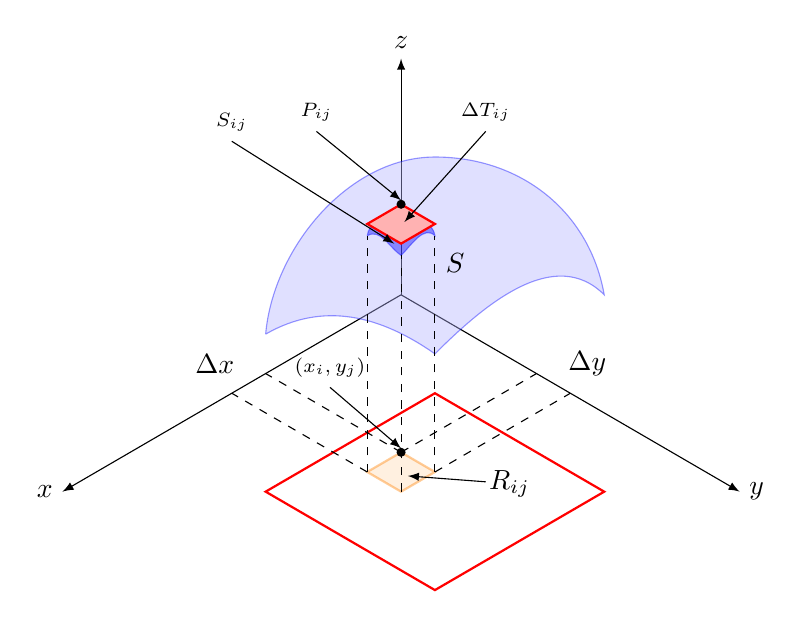
\begin{tikzpicture}[x = {(-0.86cm, -0.5cm)}, y = {(0.86cm, -0.5cm)}, 
    z = {(0cm, 1cm)}]
        \draw[-latex] (0,0,0) -- (5,0,0) node[left] {$x$};
        \draw[-latex] (0,0,0) -- (0,5,0) node[right] {$y$};
        \draw[-latex] (0,0,0) -- (0,0,3) node[above] {$z$};
        \draw[red, thick] (1, 1.5, 0) -- (3.5, 1.5, 0) -- (3.5, 4, 0) -- 
        (1, 4, 0) -- cycle;
        \node[] at (1.6, 3.2, 0) {$R_{ij}$};
        \draw[thick, orange, fill = orange!30, opacity = 0.4] (2, 2, 0) -- 
        (2, 2.5, 0) -- (2.5, 2.5, 0) -- (2.5, 2, 0) -- cycle;
        \draw[-latex] (1.75, 3, 0) -- (2.25, 2.35, 0);
        \draw[dashed] (2, 2, 0) -- (2, 0, 0);
        \draw[dashed] (2.5, 2, 0) -- (2.5, 0, 0);
        \node[] at (2.25, -0.5, 0) {$\Delta x$};
        \draw[dashed] (2, 2, 0) -- (0, 2, 0);
        \draw[dashed] (2, 2.5, 0) -- (0, 2.5, 0);
        \node[] at (-0.5, 2.25, 0) {$\Delta y$};
        \filldraw[draw = blue, fill = blue!30, opacity = 0.4] (3.5, 1.5, 2) 
        to[out = 85, in = 180, looseness = 0.9] (1, 1.5, 3) 
        to[out = 0, in = 100] (1, 4, 2.5) 
        to[out = 135, in = 45, looseness = 1] (3.5, 4, 3) 
        to[out = 145, in = 30] (3.5, 1.5, 2);
        \node[] at (3.2, 4, 4) {$S$};
        \filldraw[draw = blue, fill = blue, opacity = 0.4] (2.5, 2, 3)
        to[out = 85, in = 180, looseness = 0.9] (2, 2, 3)
        to[out = 0, in = 100] (2, 2.5, 3)
        to[out = 135, in = 45, looseness = 1] (2.5, 2.5, 3)
        to[out = 145, in = 30] (2.5, 2, 3);
        \draw[thick, red, fill = red!30] (2, 2, 3.15) -- (2, 2.5, 3.15) -- 
        (2.5, 2.5, 3.15) -- (2.5, 2, 3.15) -- cycle;
        \draw[black, fill = black] (2, 2, 0) circle (0.05cm);
        \draw[latex-] (1.95, 1.95, 0) -- (1.7, 0.65, 0) node[font = 
        \scriptsize, above] {$(x_i, y_j)$};
        \draw[dashed] (2.5, 2, 0) -- (2.5, 2, 3);
        \draw[dashed] (2.5, 2.5, 0) -- (2.5, 2.5, 3);
        \draw[dashed] (2, 2.5, 0) -- (2, 2.5, 3);
        \draw[black, fill = black] (2, 2, 3.15) circle (0.05cm);
        \draw[latex-] (1.95, 1.95, 3.15) -- (1.75, 0.5, 3.2) node[font = 
        \scriptsize, above] {$P_{ij}$};
        \draw[latex-] (2.2, 2.25, 3.15) -- (0.5, 1.75, 3.2) node[font = 
        \scriptsize, above] {$\Delta T_{ij}$};
        \draw[latex-] (2.5, 2.4, 3.1) -- (2.5, 0, 3.2) node[font = 
        \scriptsize, above] {$S_{ij}$};
    \end{tikzpicture}
    \caption{The tangent surface, $\Delta T_{ij}$, is approximately the same 
    surface area as the surface, $S_{ij}$, over the sub-rectangle, $R_{ij}$}
    \label{fig:subsurface}
\end{figure}

It follows that the total surface area of the surface, $S$, is the sum of all 
these little tangent surfaces as the number of tangent surfaces approaches 
infinity:
$$A(S) = \lim_{m, n \to \infty} \sum_{i = 1}^m \sum_{j = 1}^n \Delta T_{ij}$$

How can we find an expression for $\Delta T_{ij}$? We will define two vectors, 
\textbf{a} and \textbf{b}, that are equal to the sides of $\Delta T_{ij}$ (see 
figure \ref{fig:vectors}). Geometrically, the area of $\Delta T_{ij}$ is the 
absolute value of the cross product of the two vectors. Mathematically, 
$$\Delta T_{ij} = |\textbf{a} \times \textbf{b}|$$

\begin{figure}[htbp]
    \centering
    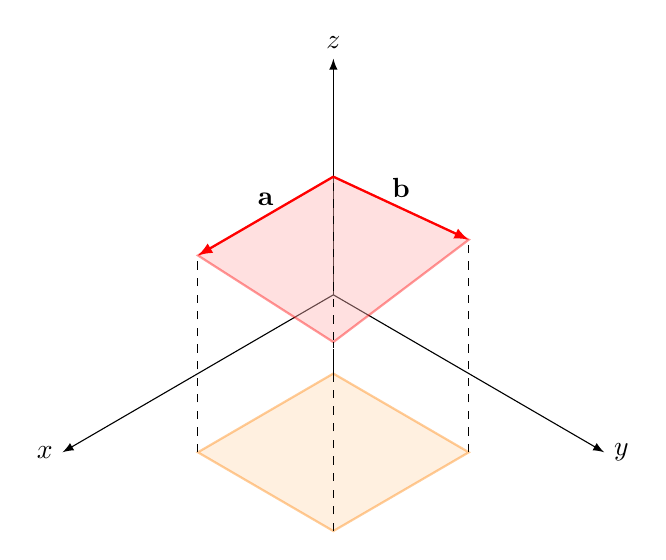
\begin{tikzpicture}[x = {(-0.86cm, -0.5cm)}, y = {(0.86cm, -0.5cm)}, 
    z = {(0cm, 1cm)}]
        \draw[-latex] (0,0,0) -- (4,0,0) node[left] {$x$};
        \draw[-latex] (0,0,0) -- (0,4,0) node[right] {$y$};
        \draw[-latex] (0,0,0) -- (0,0,3) node[above] {$z$};
        \draw[orange, thick, fill = orange!30, opacity = 0.4](1, 1, 0) -- 
        (1, 3, 0) -- (3, 3, 0) -- (3, 1, 0) -- cycle;
        \draw[red, thick, fill = red!30, opacity = 0.4] (1, 1, 2.5) -- 
        (1, 3, 2.7) -- (3, 3, 2.4) -- (3, 1, 2.5) -- cycle;
        \draw[dashed] (1, 1, 0) -- (1, 1, 2.5);
        \draw[dashed] (1, 3, 0) -- (1, 3, 2.7);
        \draw[dashed] (3, 3, 0) -- (3, 3, 2.4);
        \draw[dashed] (3, 1, 0) -- (3, 1, 2.5);
        \draw[red, thick, -latex] (1, 1, 2.5) -- (3, 1, 2.5) node[black, 
        pos = 0.5, above] {\textbf{a}};
        \draw[red, thick, -latex] (1, 1, 2.5) -- (1, 3, 2.7) node[black, 
        pos = 0.5, above] {\textbf{b}};
    \end{tikzpicture}
    \caption{The vectors \textbf{a} and \textbf{b} define the sides of the 
    tangent surface $\Delta T_{ij}$}
    \label{fig:vectors}
\end{figure}

Recall the three unit vectors: \textbf{i} in the $x$-direction, \textbf{j} in 
the $y$-direction, and \textbf{k} in the $z$-direction. We can then describe 
\textbf{a} and \textbf{b} in terms of \textbf{i}, \textbf{j}, and \textbf{k}:
$$\textbf{a} = \Delta x \textbf{i} + f_x(x_i, y_j) \Delta x \textbf{k}$$
$$\textbf{b} = \Delta y \textbf{j} + f_y(x_i, y_j) \Delta y \textbf{k}$$

(Recall that $f_x$ is the partial derivative of $f(x, y)$ with respect to $x$, 
and $f_y$ is the partial derivative with respect to $y$.) This is true because 
the partial derivative of $f_x$ gives the slope of a tangent line parallel to 
the $x$-axis, and $f_y$ parallel to the $y$-axis. We then find an expression 
for $| \textbf{a} \times \textbf{b} |$ (we've omitted some details here):
$$\textbf{a} \times \textbf{b} = -f_x(x_i, y_j) \Delta x \Delta y \textbf{i} - 
f_y(x_i, y_j) \Delta x \Delta y \textbf{j} + \Delta x \Delta y \textbf{k}$$

Substituting $\Delta A = \Delta x \Delta y$:
$$\textbf{a} \times \textbf{b} = \left[ -f_x(x_i, y_j) \textbf{i} - f_y(x_i, 
y_j) \textbf{j} + \textbf{k} \right] \Delta A$$

To find the area of $\Delta T_{ij}$, we need to find the length of $\textbf{a} 
\times \textbf{b}$. Recall that we can use the Pythagorean theorem to find the 
length of a vector. For a 3-dimensional vector $\textbf{v} = r \textbf{i} + s 
\textbf{j} + t \textbf{k}$, it's length is given by:
$$|\textbf{v}| = \sqrt{r^2 + s^2 + t^2}$$

Applying this, we find the length of $\textbf{a} \times \textbf{b}$ (which is 
the same as the area of $\Delta T_{ij}$) is:
$$\Delta T_{ij} = |\left[ -f_x(x_i, y_j) \textbf{i} - f_y(x_i, y_j) \textbf{j} 
+ \textbf{k} \right] \Delta A|$$
$$= \sqrt{\left(-f_x(x_i, y_j) \Delta A \right)^2 + \left( - f_y(x_i, y_j) 
\Delta A \right)^2 + \left( \Delta A \right)^2}$$
$$= \sqrt{\left[ f_x(x, y)\right]^2 + \left[f_y(x, y) \right]^2 + 1} \Delta A$$

So, the area of the entire surface over region \textit{R} is:
$$A(S) = \lim_{m, n \to \infty} \sum_{i = 1}^m \sum_{j = 1}^n \sqrt{\left[ f_x(
x, y)\right]^2 + \left[f_y(x, y) \right]^2 + 1} \Delta A$$

This is the definition of a double integral; therefore, the surface area of 
a two-variable function, $f(x, y)$ over a region, $R$, where $f_x$ and $f_y$ 
are continuous, is:
$$A(S) = \iint_{\textit{R}} \sqrt{\left[ f_x(x, y)\right]^2 + \left[f_y(x, y) 
\right]^2 + 1}\,dA$$

Using the notation of partial derivatives, this is also expressed as:
$$A(S) = \iint_{\textit{R}} \sqrt{1 + \left( \frac{\partial z}{\partial x} 
\right)^2 + \left( \frac{\partial z}{\partial y} \right)^2}\,dA$$

\textbf{Example}: Find the surface area of the part of the surface $z = 2 - 
y^2$ that lies over the triangle whose vertices are at $(0, 0)$, $(0, 4)$, and 
$(3, 4)$. 

\textbf{Solution}: We can define $\textit{R} = \{(x, y)\text{ }|\text{ }0 \leq 
x \leq {3}{4}y,\text{ }0 \leq y \leq 4\}$. Additionally, 
$$\frac{\partial z}{\partial x} = 0$$
$$\frac{\partial z}{\partial y} = -2y$$

Therefore, the area of the surface that lies above \textit{R} is:
$$A(S) = \iint_{\textit{R}} \sqrt{1 + 0^2 + \left( -2y \right)^2}\,dA = 
\int_0^4 \int_0^{\frac{3}{4}y} \sqrt{1 + 4y^2}\,dx\,dy$$
$$= \int_0^4 \sqrt{1 + 4y^2} \left[ x \right]_{x = 0}^{x = \frac{3}{4}y}\,dy 
= \frac{3}{4} \int_0^4 y \sqrt{1 + 4y^2}\,dy$$

Let $u = 1 + 4y^2$, then $du = (8y)dy$ and $(y)dy = \frac{du}{8}$. Substituting:
$$A(S) = \frac{3}{4} \int_{y = 0}^{y = 4} \frac{1}{8} \sqrt{u}\,du = \frac{3}{
32} \left[ \frac{2}{3} u^{3/2} \right]_{y = 0}^{y = 4}$$
$$= \frac{1}{16} \left[ \left(1 + 4y^2 \right)^{3/2} \right]_{y = 0}^{y = 4} = 
\frac{1}{16} \left[ \left( 65 \right)^{3/2} - 1 \right] \approx 32.69$$

\begin{Exercise}[title = {Surface Area of Two-Variable Functions}, label = 
surface]
Find the area of the surface.
\begin{enumerate}
\item The part of the plane $9x + 6y - 3z + 6 = 0$ that lies above the 
rectangle $\left[2, 6 \right] \times \left[1, 4 \right]$.
\item The part of the paraboloid in the circle $z = 2x^2 + 2y^2$ that lies 
under the plane $z = 32$. 
\item The part of the surface $z = 3xy$ that lies in the cylinder $x^2 + y^2 
= 4$.
\end{enumerate}
\end{Exercise}

\begin{Answer}[ref = surface]
\begin{enumerate}
\item Rearranging the formula for the plane, we find that $z = 3x + 2y + 2$. Therefore, $\partial z / \partial x = 3$ and $\partial z / \partial y = 2$. 
Then the surface area is given by:
$$A(S) = \int_2^6 \int_1^4 \sqrt{1 + 3^2 + 2^2}\,dy\,dx = \int_2^6 \sqrt{14}y|_
{y = 1}^{y = 4}\,dx$$
$$= \int_2^6 3\sqrt{14}\,dx = 3\sqrt{14}x|_{x = 2}^{x = 6} = 12\sqrt{14}$$
\item The paraboloid intersects the plane when $2x^2 + 2y^2 = 32$, which is the
circle of radius 4 centered at the origin. So, we are looking for the area of 
the surface $z = 2x^2 + 2y^2$ that lies above the region $\textit{R} - \{(r, 
\theta)\text{ }|\text{ }0 \leq r \leq 4,\text{ } 0 \leq \theta \leq 2\pi \}$. 
The surface area is:
$$A(S) = \iint_{\textit{R}} \sqrt{1 + \left(4x \right)^2 + \left( 4y \right)^2}
\,dA = \int_0^4 \int_0^{2\pi} r \sqrt{1 + \left(4 r \cos{\theta} \right)^2 + 
\left( 4 r \sin{\theta} \right)^2}\,d\theta\,dr$$
$$= \int_0^4 \int_0^{2\pi} r \sqrt{1 + 16r^2}\,d\theta\,dr = \int_0^4 r \sqrt{
1 + 16r^2} \left[\theta \right]_{\theta = 0}^{\theta = 2\pi}\,dr$$
$$= \int_0^4 2\pi r \sqrt{1 + 16r^2}\,dr$$

Let $u = 1 + 16r^2$, then $du = 32r (dr)$ and $r(dr) = du/32$. Substituting:
$$A(S) = \frac{2\pi}{32} \int_{r = 0}^{r = 4} \sqrt{u}\,du = \frac{\pi}{16} 
\left( \frac{2}{3} \right) \left[u^{3/2} \right]_{r = 0}^{r = 4}$$
$$= \frac{\pi}{24} \left[ \left(1 + 16r^2 \right)^{3/2} \right]_{r = 0}^{r = 4}
= \frac{\pi}{24} \left[ \left(257 \right)^{3/2} - 1\right] \approx 6470.15$$

\item The region, \textit{R}, we are interested in is the circle of radius 2 
centered at the origin of the $xy$-plane, described by $\textit{R} = \{(r, 
\theta)\text{ }|\text{ }0 \leq r \leq 2,\text{ }0 \leq \theta \leq 2\pi \}$. 
Noting that $\partial z / \partial x = 3y$ and $\partial z / \partial y = 3x$, 
we see that the surface area is given by:
$$A(S) = \iint_{\textit{R}} \sqrt{1 + \left(3y \right)^2 + \left( 3x \right)^2}
\,dA = \int_0^2 \int_0^{2\pi} r \sqrt{1 + 9r^2\sin^2{\theta} + 9r^2\cos^2{
\theta}}\,d\theta\,dr$$
$$= \int_0^2 \int_0^{2\pi} r \sqrt{1 + 9r^2}\,d\theta\,dr = 2\pi \int_0^2 r 
\sqrt{1 + 9r^2}\,dr$$

Let $u = 1 + 9r^2$, then $du = 18r(dr)$, which means that $r(dr) = du/18$. 
Substituting:
$$A(S) = \frac{2\pi}{18} \int_{r = 0}^{r = 2} \sqrt{u}\,du = \frac{\pi}{9} 
\left( \frac{2}{3} \right) \left[ u^{3/2} \right]_{r = 0}^{r = 2}$$
$$= \frac{2\pi}{27} \left[ \left(1 + 9(4) \right)^{3/2} - 1 \right] = \frac{2
\pi}{27} \left[ \left(37 \right)^{3/2} - 1 \right] \approx 52.14$$
\end{enumerate}
\end{Answer}

\section{Average Value}
Recall that the average value of a one-variable function over the interval $x 
\in [a, b]$ is given by:
$$f_{ave} = \frac{1}{a - b}\int_a^b f(x)\,dx$$

For a two-variable function, the average value over a region, $R$, is given by:
$$f_{ave} = \frac{1}{A(R)} \iint_{R} f(x, y)\,dA$$

Where $A(R)$ is the area of the two-dimensional region. 

\textbf{Example}: Find the average value of $f(x, y) = xy^2$ over the rectangle
with vertices at $(-2, 0)$, $(-2, 4)$, $(2, 4)$, and $(2, 0)$. 

\textbf{Solution}: The rectangular region has an area of $(2 - (-2)) \cdot (4 -
0) = 4 \cdot 4 = 16$. Therefore, the average value is given by:
$$f_{ave} = \frac{1}{16} \iint_{R} xy^2\,dA = \frac{1}{16} \int_{-2}^2 \int_0^4
xy^2\,dy\,dx$$
$$= \frac{1}{16} \int_{-2}^2 \frac{x}{3} y^3|_{y = 0}^{y = 4}\,dx = \frac{1}{
16} \int_{-2}^2 \frac{x}{3} \left(4^3 \right)\,dx = \frac{4}{3} \int_{-2}^2 x\,
dx$$
$$= \frac{4}{3} \left( \frac{1}{2} \right) x^2|_{x = -2}^{x = 2} = 0$$

\begin{Exercise}[title = {Average Value}, label = avg]
Find the average value of the function over the region \textit{D}:
\begin{enumerate}
\item $f(x, y) = x\sin{y}$, $\textit{D} = [0, 2] \times [-\pi/2, \pi/2]$
\item $f(x, y) = x + y$, \textit{D} is the circle with radius 1 centered at 
$(1, 0)$
\item $f(x, y) = xy$, \textit{D} is the triangle with vertices at $(0, 0)$, 
$(2, 0)$, $(2, 2)$
\end{enumerate}
\vspace{70mm}
\end{Exercise}

\begin{Answer}[ref = avg]
\begin{enumerate}
\item The area of \textit{D} is $2\pi$. Therefore, the average value is:
$$\frac{1}{2\pi} \iint_{\textit{D}} x\sin{y}\,dA = \frac{1}{2\pi} \int_0^2 
\int_{0}^{\pi} x\sin{y}\,dy\,dx$$
$$= \frac{1}{2\pi} \int_0^2 -x\cos{y}|_{y = 0}^{y = \pi}\,dx = \frac{1}{2\pi} 
\int_0^2 -x \left( \cos{\pi} - \cos{0} \right)\,dx$$
$$= \frac{1}{2\pi} \int_0^2 (-x)(-1 - 1)\,dx = \frac{1}{2\pi} \int_0^2 2x\,dx$$
$$= \frac{1}{2\pi} x^2|_{x = 0}^{x = 2} = \frac{2}{\pi}$$
\item Since \textit{D} is a circle of radius $r = 1$, the area is $A = \pi r^2 
= \pi$. \textit{D} can be described with $\textit{D} = \{ (r, \theta)\text{ }|
\text{ } 0 \leq r \leq 2\cos{\theta},\text{ } -\pi/2 \leq \theta \leq \pi/2\}$.
Therefore, the average value of $f(x, y) = x + y$ over \textit{D} is:
$$f_{ave} = \frac{1}{\pi} \iint_{\textit{D}} \left(x + y \right)\,dA = 
\frac{1}{\pi} \int_{-\pi/2}^{\pi/2} \int_0^{2\cos{\theta}} r \cdot \left(r\cos{
\theta} + r\sin{\theta} \right)\,dr\,d\theta$$
$$= \frac{1}{\pi} \int_{-\pi/2}^{\pi/2} \left(\cos{\theta} + \sin{\theta} 
\right) \left[\int_0^{2\cos{\theta}} r^2 \,dr \right]\,d\theta$$
$$= \frac{1}{\pi} \int_{-\pi/2}^{\pi/2} \left(\cos{\theta} + \sin{\theta} 
\right) \cdot \left[ \frac{1}{3} r^3 \right]_{r = 0}^{r = 2\cos{\theta}}\,d
\theta$$
$$= \frac{8}{3\pi} \int_{-\pi/2}^{\pi/2} \left(\cos{\theta} + \sin{\theta} 
\right) \cos^3{\theta}\,d\theta = \frac{8}{3\pi} \int_{\pi/2}^{\pi/2} \left( 
\cos^4{\theta} + \sin{\theta} \cos^3{\theta} \right)\,d\theta$$
$$= \frac{8}{3\pi} \left[ \int_{-\pi/2}^{\pi/2} \left( \frac{1 + \cos{2
\theta}}{2} \right)^2\,d\theta - \left[ \frac{1}{4} \cos^4{\theta} \right]_{
\theta = -\pi/2}^{\theta = \pi/2} \right]$$
$$= \frac{2}{3\pi} \int_{-\pi/2}^{\pi/2} \left(1 + 2\cos{2\theta} + \cos^2{2
\theta} \right)\,d\theta = \frac{2}{3\pi} \left[ \left(\theta + \sin{2\theta} 
\right)_{\theta = -\pi/2}^{\theta = \pi/2} + \int_{-\pi/2}^{\pi/2} \frac{1 + 
\cos{4\theta}}{2}\,d\theta \right]$$
$$= \frac{2}{3\pi} \left[ \pi + \frac{1}{2} \left(\theta + \frac{1}{4}\sin{4
\theta} \right)_{\theta = -\pi/2}^{\theta = \pi/2} \right] = \frac{2}{3\pi} 
\left[ \pi + \frac{1}{2} \left( \pi \right) \right] = \frac{2}{3\pi} \left( 
\frac{3\pi}{2} \right) = 1$$
\item Let's visualize \textit{D}:

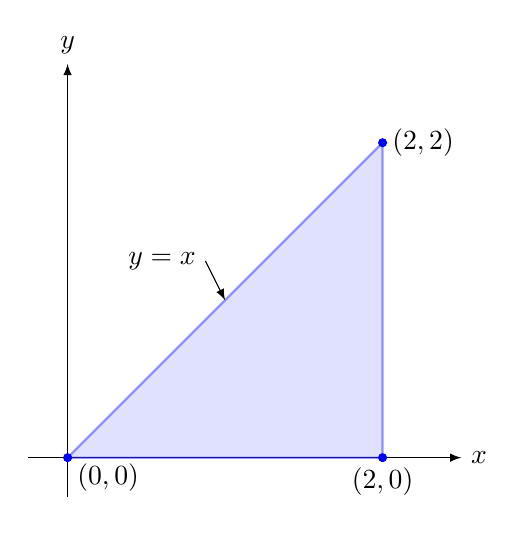
\begin{tikzpicture}
    \draw[-latex] (-0.5, 0) -- (5, 0) node[right] {$x$};
    \draw[-latex] (0, -0.5) -- (0, 5) node[above] {$y$};
    \draw[blue, thick, fill = blue!30, opacity = 0.4] (0,0) -- (4, 0) -- 
    (4,4) -- cycle;
    \draw[latex-] (2,2) -- (1.75, 2.5) node[left] {$y = x$};
    \draw[blue, fill = blue] (0,0) circle (0.05cm) node[black, right, yshift = 
    -0.25cm] {$(0, 0)$};
    \draw[blue, fill = blue] (4, 0) circle (0.05cm) node[black, below] {
    $(2, 0)$};
    \draw[blue, fill = blue] (4, 4) circle (0.05cm) node[black, right] {
    $(2, 2)$};
\end{tikzpicture}

So, \textit{D} can be described $\textit{D} = \{(x, y)\text{ }|\text{ }0 \leq 
x \leq 2,\text{ }0 \leq y \leq x\}$. Additionally, \textit{D} has area $A = 
\frac{1}{2} \left( 2^2 \right) = 2$. Therefore, the average value of $f(x,y) = 
xy$ over \textit{D} is:
$$f_{ave} = \frac{1}{2} \iint_{\textit{D}} \left(xy \right)\,dA = \frac{1}{2} 
\int_0^2 \int_0^x \left(xy \right)\,dy\,dx$$
$$= \frac{1}{2} \int_0^2 x \left[ \frac{1}{2}y^2 \right]_{y = 0}^{y = x}\,dx = 
\frac{1}{4} \int_0^2 x^3\,dx = \frac{1}{4} \left[ \frac{1}{4}x^4 \right]_{x = 0
}^{x = 2}$$
$$= \frac{1}{16} \left(2^4 \right) = 1$$
\end{enumerate}
\end{Answer}

